\documentclass[journal, a4paper]{IEEEtran}
\usepackage{cite}
\usepackage{amsmath,amssymb,amsfonts}
\usepackage{graphicx}
\usepackage{textcomp}
\usepackage{xcolor}
\usepackage{float}

\begin{document}

\title{Explaining the Black Box: A Study on the Application of Explainable Artificial Intelligence (XAI) Techniques to Machine Learning Models}
\author{
    \large
    \IEEEauthorblockN{Magdalena~Pakuła\IEEEauthorrefmark{1}}
    and
    \IEEEauthorblockN{Jakub~Pawlak\IEEEauthorrefmark{2}}\\[1ex]
    \normalsize
    \IEEEauthorblockA{
        WFTIMS, Politechnika Łódzka\\
        Email: \IEEEauthorrefmark{1}254220@edu.p.lodz.pl, \IEEEauthorrefmark{2}254222@edu.p.lodz.pl
    }
}


\maketitle

\begin{abstract}
    The increasing reliance on artificial neural networks in various applications has raised concerns about their \textit{black box} nature, making it challenging to understand the decision-making processes behind their predictions.
    This report addresses this challenge by exploring the application of so-called Explainable Artificial Intelligence (XAI) techniques to machine learning models.
    Specifically, we employ local explanation approaches, including attributions and counterfactual examples, using the Captum library in the PyTorch such as LIME, saliency maps or MinParamPerturbation techniques.
    Our study aims to shed light on the previously trained models, providing a deeper understanding of how they make predictions and present those findings in this report
\end{abstract}

\section{Introduction}\label{sec:introduction}

\IEEEPARstart{A}{rtificial} neural networks have revolutionized various industries and applications, from healthcare to finance, by enabling accurate predictions and decision-making.
However, the increasing reliance on these models has also raised concerns about their \textit{black box} nature, making it challenging to understand the decision-making processes behind their predictions.
This opacity can lead to a lack of trust in the models, as well as difficulties in identifying biases and errors.
To address this challenge, Explainable Artificial Intelligence (XAI) techniques have emerged as a crucial step towards building more transparent and accountable machine learning models.
By applying XAI methods, we can gain insights into the internal workings of complex models, providing a deeper understanding of how they make predictions and enabling more informed decision-making.
This project aims to explore the application of XAI techniques to machine learning models, specifically focusing on local explanation approaches such as attributions and counterfactual examples.
By shedding light on the previously trained models, we aim to provide a better understanding of how they make predictions and contribute to the development of more transparent and trustworthy AI systems.

\section{Related Work}\label{sec:related-work}

One of the first work in this paper's domain is~\cite{ribeiro2016should} by Ribeiro et al.
This is the first paper introducing LIME (Local Interpretable Model-Agnostic Explanations) framework, which generates local, interpretable explanations for the predictions of any machine learning model.
Another influential text is the book~\cite{molnar2019interpretable} by Christoph Molnar, which provides an overview of various XAI techniques, including feature importance, partial dependence plots, and SHAP values.
Molnar discusses both global and local explanation methods, highlighting their strengths, weaknesses, and appropriate use cases.
The last paper~\cite{samek2017explainable} by Samek et al.\ offers a broader perspective on the field of XAI\@.
The authors present a taxonomy of XAI techniques, categorizing them into different groups based on their underlying principles and goals.
The paper also discusses the opportunities and challenges in developing XAI systems.

Those papers provide a solid ground for understanding the importance of interpretability and explainability in machine learning.
However, there is still a need for further experimentation and evaluation on diverse datasets and scenarios to better understand the strengths and limitations of different XAI approaches.

\section{Methods}\label{sec:methodology}

This experiment will be conducted on varius types of data and different models.
Those models are: MLP models for classifying iris flowers, distinguishing wines and diagnosing breast cancer, MLP models and CNN network for classifying handwritten numbers from the MNIST dataset and lastly CNN network for distinguishing objects in images from the CIFAR10 dataset.

Based on the research, general knowledge, and the types of data and models involved, the experiment will utilize a combination of local and global explanation methods to provide insights into the inner workings of these machine learning systems.

\subsection{Explainable AI Techniques}\label{subsec:explainable-ai-techniques}

For local explanations, the following techniques will be employed:

\begin{itemize}
    \item \textbf{LIME}: This method learns an interpretable model around the prediction, allowing for an understanding of the key factors driving the model's output for a specific instance. LIME is a suitable choice as it is a model-agnostic approach that can be applied to a wide range of machine learning models, including the MLP and CNN architectures used in this experiment.
    \item \textbf{Saliency Maps}: Saliency maps highlight the input features that have the most significant influence on the model's prediction for a given instance. This technique is particularly useful for understanding the decision-making process of the CNN models used for image classification tasks, as it can identify the salient regions of the input images that are driving the predictions.
    \item \textbf{Minimal Parameter Perturbation}: This counterfactual explanation method identifies the minimal changes required to the input features to change the model's prediction. By understanding the necessary perturbations, we can gain insights into the model's decision boundaries and the key factors contributing to its predictions.
\end{itemize}

In addition to these local explanation methods, the experiment will also explore global explanations to understand the overall behavior and assumptions of the trained models.

\subsection{Experiments}\label{subsec:experiments}

\section{Results}\label{sec:results}
Present the results of the local and global explanations.
Interpret the findings, discuss their significance, and potential implications.

\subsection{Iris MLP classifier}\label{subsec:experiment-iris}
\subsection{Wine MLP classifier}\label{subsec:experiment-wine}
\subsection{Breast cancer MLP classifier}\label{subsec:experiment-cancer}

\subsection{MNIST MLP classifier}\label{subsec:experiment-mnist-mlp}

\subsubsection{Flatten}
\subsubsection{LBP}
\subsubsection{HOG}

\subsection{MNIST CNN classifier}\label{subsec:experiment-mnist-cnn}

\begin{figure}[ht]\centering
    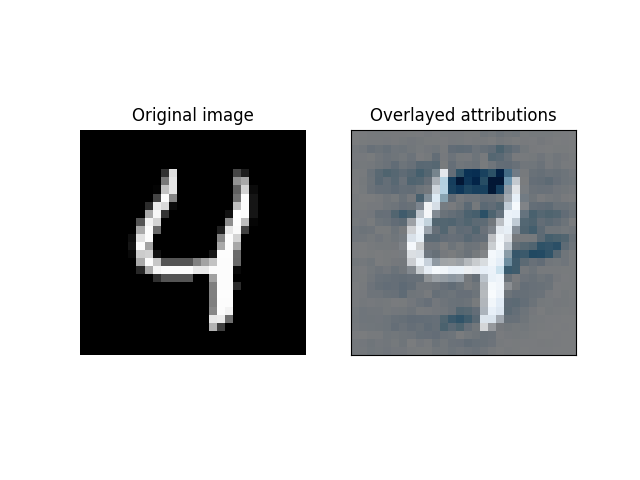
\includegraphics[width=.6\linewidth]{img/saliency_mnist/4.png}
    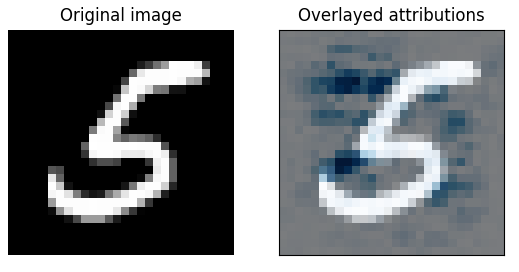
\includegraphics[width=.6\linewidth]{img/saliency_mnist/5.png}
    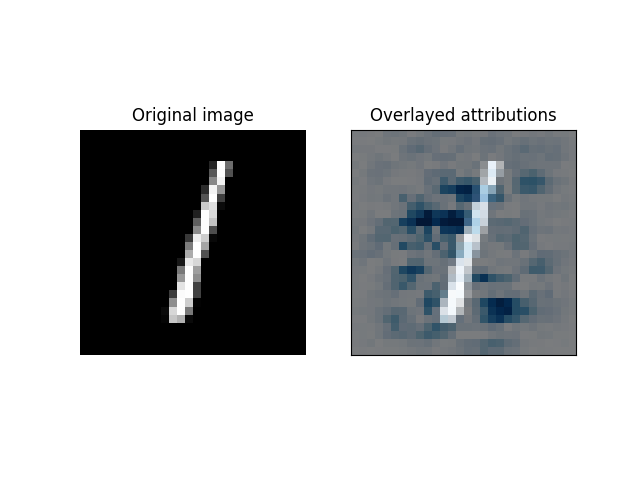
\includegraphics[width=.6\linewidth]{img/saliency_mnist/1.png}
    \caption{Saliency maps of chosen MNIST digits}\label{fig:mnist-cnn-saliency}
\end{figure}

The CNN for recognizing handwritten digits from the MNIST dataset was analyzed using the saliency methods.
The resulting saliency maps are visualized on fig.~\ref{fig:mnist-cnn-saliency}.
The blue pixels show the areas that most influence the model's predictions.

Unexpectedly, the obtained saliency maps predominantly highlight background pixels adjacent to the digits
rather than the digits themselves.
One plausible explanation of this phenomenon is that the CNN has learned the absence of pixels in a specific region as
impotant information for its classification decisions --- for example, the digits 4 and 5 are characterized by the lack of the closed regions.
If one was to add pixels to these areas 4 would turn into a 9, and 5 would turn into a 6.
Therefore, these areas are highlited as important to the classification results, because it is essential that no pixels exist in those areas.
Such behaviour might suggest that the model is not recognizing the digits by their shape directly, but rather by ellimination --- i.e.\ an important characteristic of a digit 4 is that it is not a 9.

The background pixels might also provide contextual information about the area around the digit.
This is especially importnant in shape recognition tasks, such as digit recognition.
For example, the top bar at the digit 5 is oriented to the right-hand side, however, there are pixels highlited to the left-hand side.
That is because for a line to be considered as oriented to the right, there need to be both a presence of pixels to the right, and a lack of them to the left.
Therefore, the background also needs to be considered in order to correctly determine the shape characteristics and boundaries.

Another unfortunate possibility of such behaviour may be some issues with the model.
Overfitting could cause the model to focus on some background pixels, that are not really representative of the digit features.
However, it should be noted that during the model evaluation, we did not observe a drop in accuracy on the test set during training --- a typical sign of overfitting.
Additionally, the performance of the model on the testing data was satisfactory, which speaks against the potential issues with the model.


\subsection{CIFAR10 CNN classifier}\label{subsec:experiment-cifar}

\section{Summary}\label{sec:summary}
Summarize the main conclusions and suggest future work.

\section{References}\label{sec:references}

\bibliographystyle{IEEEtran}
\bibliography{references}

\end{document}
